\documentclass[a4paper]{article}
\usepackage{graphicx}
\usepackage[a4paper, left=5mm, right=5mm, top=5mm, bottom=5mm]{geometry}
%\geometry{paperwidth=210mm, paperheight=2000pt, left=5pt, top=5pt}
\usepackage[utf8]{inputenc}
\usepackage[english,russian]{babel}
\usepackage{indentfirst}
\usepackage{tikz} %Рисование автоматов
\usetikzlibrary{automata,positioning,arrows,trees,calc}
\usepackage{amsmath}
\usepackage[makeroom]{cancel} % зачеркивание
\usepackage{multicol,multirow} %Несколько колонок
\usepackage{hyperref}
\usepackage{tabularx}
\usepackage{amsfonts}
\usepackage{wrapfig}
\usepackage{amssymb}
\DeclareMathOperator*{\argmin}{arg\,min}
\usepackage{listings}
\usepackage{wasysym}
\date{2014.12.25}
\author{Сергей~Володин, 274 гр.}
\newcommand{\matrixl}{\left|\left|}
\newcommand{\matrixr}{\right|\right|}
% названия автоматов  (rubtsov)
\def\A{{\cal A}}
\def\B{{\cal B}}
\def\C{{\cal C}}

\title{Эффект Эйнштейна --- де Хааза\\(реферат)}

%+= и -=, иначе разъезжаются...
\newcommand{\peq}{\mathrel{+}=}
\newcommand{\meq}{\mathrel{-}=}
\newcommand{\deq}{\mathrel{:}=}
\newcommand{\plpl}{\mathrel{+}+}

% пустое слово  (rubtsov)
\def\eps{\varepsilon}

\def\eqdef{\overset{\mbox{\tiny def}}{=}}
\newcommand{\niton}{\not\owns}


\newcommand{\smalll}[1]{\overline{\overline{#1}}}
\newcommand{\smallo}{\bar{\bar{o}}}
\begin{document}
\maketitle
\section*{Введение}
В 1820 году Эрстед выяснил, что магнитное поле может быть создано не только постоянными магнитами, но еще и токами. Получалось, что источников магнитного поля может быть два типа: токи и постоянные магниты. В попытке разобраться в этой ситуации и выяснить природу магнетизма, сведя два типа к одному, Ампер выдвинул гипотезу, согласно которой в постоянных магнитах циркулируют без сопротивления молекулярные токи, которые и создают магнитное поле. В 1915 году Эйнштейн и де Хааз провели эксперимент, подтверждающий гипотезу Ампера.

В модели атома Бора (1913) электрон вращается по круговой орбите. Из-за этого, во-первых, он имеет момент импульса, во-вторых, магнитный момент, так как электрон~--- заряженная частица. Поэтому следует ожидать, что изменение магнитных свойств (намагничивание) будет приводить к изменению механических: тело начнет вращаться. Такой эффект и наблюдали Эйнштейн и де Хааз.
\section*{Классическое обоснование (модель Бора, орбитальный момент)}
Рассмотрим атом модели Бора. Электрон с зарядом $e=-1.6\cdot 10^{-19}$ Кл движется вокруг ядра с зарядом $Z|e|$. Момент импульса электрона $L=mvr=m\frac{2\pi r}{T}r=m 2\pi r^2 \nu,$ где $\nu$~--- частота обращения электрона вокруг ядра. Магнитный момент $M=IS=e\nu\pi r^2$. Отсюда получаем гиромагнитное отношение $\gamma\eqdef \frac{M}{L}=\frac{e\nu\pi r^2}{2m\pi\nu r^2}=\frac{e}{2m}\approx -8.79\cdot 10^{10}\frac{\mbox{Кл}}{\mbox{кг}}$. Обратная величина $\frac{1}{\gamma}=-1.14\cdot 10^{-11}\frac{\mbox{кг}}{\mbox{Кл}}$.

В векторном виде гиромагнитное соотношение записывается как $\vec{M}=\gamma\vec{L}$

Из-за наличия такого соотношения изменение намагниченности образца приведет к его вращению как целого. Действительно, пусть $\vec{L}_1$~--- сумма всех орбитальных моментов импульса электронов, $\vec{L}_2$~--- момент импульса тела как целого. Полный момент сохраняется: $0=\frac{d}{dt}(\vec{L}_1+\vec{L}_2)$, откуда $\frac{d\vec{L}_2}{dt}=-\frac{d\vec{L}_1}{dt}=-\frac{1}{\gamma}\frac{d}{dt}\sum\limits_i \vec{M}_i$, где $\vec{M}_i$~--- орбитальные магнитные моменты всех атомов. Это можно интерпретировать так: на тело как целое действует момент силы $\vec{\tau}=-\frac{1}{\gamma}\frac{d}{dt}\vec{M}_\Sigma$., то есть, тело начнет вращаться.

Пусть внешнее магнитное поле изменяется с $\vec{B}_0$ до противоположного $-\vec{B}_0$. Пусть $B_0$ достаточно сильное, т.е. намагниченность достигает насыщения и изменяется с $\vec{I}s$ на противоположное $-\vec{I}_s$. Изменение момента импульса $J\Delta \omega=\int\limits_0^t\tau dt=\int\limits_0^t -\frac{1}{\gamma}\frac{d}{dt}(M_\Sigma) dt=-\frac{\Delta M_\Sigma}{\gamma}$. Тогда $\Delta\omega=-\frac{4I_s}{\gamma\rho R^2}\approx 0.6\cdot 10^{-8}\mbox{с}^{-1}$, если взять $J=\frac{1}{2}MR^2$, $R=10^{-3}\mbox{м}$, $I_s=1\mbox{Тл}$, $\rho=7800\frac{\mbox{кг}}{\mbox{м}^3}$.

\section*{Эксперимент}
\begin{figure}
	\begin{center}
		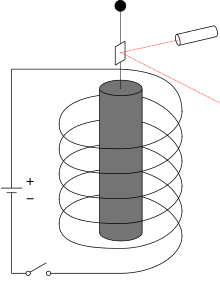
\includegraphics[width=5cm]{lab.png}
	\end{center}
\end{figure}
\begin{wrapfigure}{r}{0.5\textwidth}
	\begin{center}
		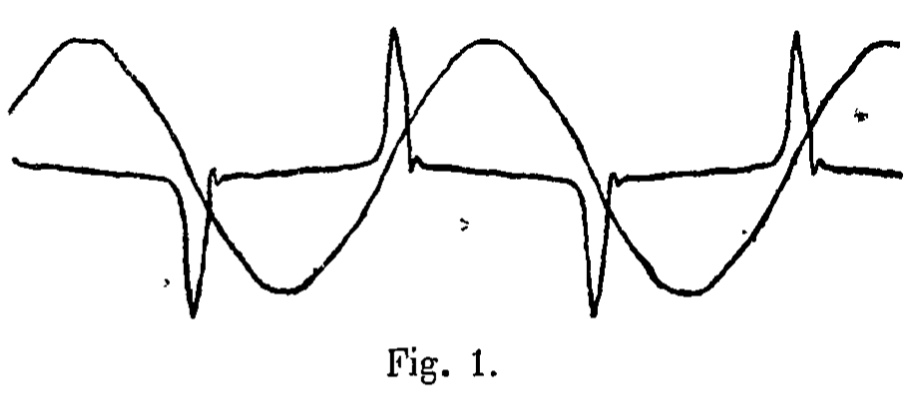
\includegraphics[width=5cm]{fig1.png}
		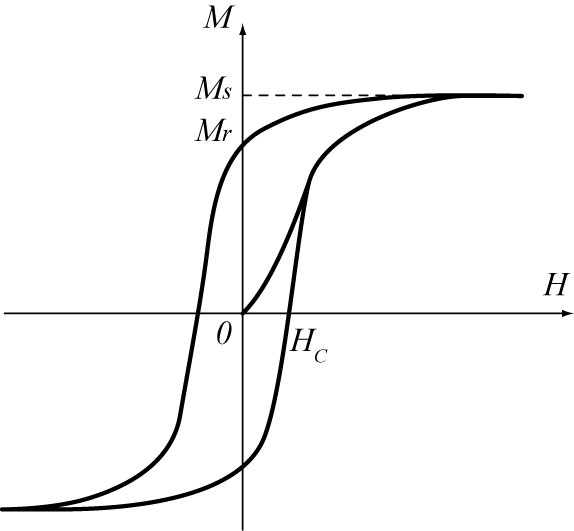
\includegraphics[width=5cm]{hyst.jpg}
	\end{center}
\end{wrapfigure}
Рассмотрим подвешенный на нити цилиндр, помещенный в катушку с током $i$, которая создает магнитное поле. Запишем уравнение колебаний:
$$\ddot{\alpha}+2\beta\dot{\alpha}+\omega_0^2\alpha=\frac{1}{J}\tau$$
Пропустим через катушку синусоидальный ток частоты $\omega$. Момент сил $\tau$ в таком случае не обязан быть синусоидальным, так как кривая намагничивания нелинейна (петля гистерезиса) при достаточно больших внешних полях, а именно такие поля и были использованы. Эйнштейном и де Хаазом был получен график зависимости тока от времени и момента сил от времени. Ток синусоидальный, а момент сил (вторая кривая)~--- нет.\newline
<<Пик>> возникает при смене знака тока, что соответствует смене знака внешнего магнитного поля, т.е. движению вдоль кривой гистерезиса вблизи нуля, где производная $\frac{dI}{dt}$ как раз велика. <<Плоские>> участки соответствую движению по асимптотам (насыщение).
Выражение для тока $i=A\sin\omega t$. Разложим момент сил в ряд Фурье на периоде $T=\frac{2\pi}{\omega}$ как четную функцию: $\tau=\sum\limits_{n=1}^{\infty}B_n\cos n\omega t$. В результирующих колебаниях амплитуда велика только для первого члена при $\omega\approx\omega_0$ (резонанс). Вычислим $B_1$. На отрезке $t\in[-\frac{\pi}{2\omega},\frac{3\pi}{2\omega}]$ наблюдается два пика, первый вверх, второй вниз. Проинтегрируем разложение для момента, умноженное на $\cos\omega t$ по указанному периоду (<<перекрестные>> члены уйдут): $$\int\limits_{-\frac{\pi}{2\omega}}^{\frac{3\pi}{2\omega}}\tau\cos\omega tdt=\int\limits_{-\frac{\pi}{2\omega}}^{\frac{3\pi}{2\omega}}B_1\cos^2\omega tdt=\frac{\pi}{\omega}B_1$$

В первом пике ($t\approx0$) значение $\cos\omega t\approx 1$, во втором пике ($t\approx \frac{\pi}{\omega}$) значение $\cos\omega t\approx -1$. Интеграл по каждому пику, как показано выше, равен $\int \tau dt=-\frac{2}{\gamma}M_s$, где $M_s=I_sV$~--- суммарный магнитный момент при насыщении. В итоге интеграл слева можно оценить как $-\frac{4}{\gamma}I_sV$. Получаем соотношение $B_1=-\frac{4I_sV\omega}{\pi\gamma}$.

Найдем решение уравнения колебаний, оставим только член с $\cos\omega t$ (резонансный):
$$
\frac{B_1}{J}\cos\omega t=\ddot{\alpha}+2\beta\dot{\alpha}+\omega_0^2\alpha
$$
Собственные колебания не учитываем, так как они затухающие (ими можно пренебречь). Частное решение ищем в виде $\alpha(t)=\mbox{Re} Ae^{i\omega t}$, получаем $A=\frac{B_1/J}{(\omega_0^2-\omega^2)+2\beta i\omega}$
\begin{thebibliography}{}
\item В.Я.Френкель. УФН т.128, (1979) с.545.
\item A. Einstein, W. J. de Haas, Experimental proof of the existence of Ampère's molecular currents (in English), Koninklijke Akademie van Wetenschappen te Amsterdam, Proceedings, 18 I, pp. 696–711 (1915).
\end{thebibliography}
\end{document}